%%%%%%%%%%%%%%%%%%%%%%%%%%%%%%%%%%%%%%%%%
% Beamer Presentation
% LaTeX Template
% Version 1.0 (10/11/12)
%
% This template has been downloaded from:
% http://www.LaTeXTemplates.com
%
% License:
% CC BY-NC-SA 3.0 (http://creativecommons.org/licenses/by-nc-sa/3.0/)
%
%%%%%%%%%%%%%%%%%%%%%%%%%%%%%%%%%%%%%%%%%

%----------------------------------------------------------------------------------------
%	PACKAGES AND THEMES
%----------------------------------------------------------------------------------------

\documentclass[UTF8,aspectratio=169,14pt]{ctexbeamer}

\usepackage{hyperref}
\hypersetup{
	colorlinks=true,
	linkcolor=red,
	anchorcolor=blue,
	citecolor=green
}

\mode<presentation> {
	
	% The Beamer class comes with a number of default slide themes
	% which change the colors and layouts of slides. Below this is a list
	% of all the themes, uncomment each in turn to see what they look like.
	
	%\usetheme{default}
	%\usetheme{AnnArbor}
	%\usetheme{Antibes}
	%\usetheme{Bergen}
	%\usetheme{Berkeley}
	%\usetheme{Berlin}
	%\usetheme{Boadilla}
	%\usetheme{CambridgeUS}
	%\usetheme{Copenhagen}
	%\usetheme{Darmstadt}
	%\usetheme{Dresden}
	%\usetheme{Frankfurt}
	%\usetheme{Goettingen}
	%\usetheme{Hannover}
	%\usetheme{Ilmenau}
	%\usetheme{JuanLesPins}
	%\usetheme{Luebeck}
	\usetheme{Madrid}
	%\usetheme{Malmoe}
	%\usetheme{Marburg}
	%\usetheme{Montpellier}
	%\usetheme{PaloAlto}
	%\usetheme{Pittsburgh}
	%\usetheme{Rochester}
	%\usetheme{Singapore}
	%\usetheme{Szeged}
	%\usetheme{Warsaw}
	
	% As well as themes, the Beamer class has a number of color themes
	% for any slide theme. Uncomment each of these in turn to see how it
	% changes the colors of your current slide theme.
	
	%\usecolortheme{albatross}
	%\usecolortheme{beaver}
	%\usecolortheme{beetle}
	%\usecolortheme{crane}
	%\usecolortheme{dolphin}
	%\usecolortheme{dove}
	%\usecolortheme{fly}
	%\usecolortheme{lily}
	%\usecolortheme{orchid}
	%\usecolortheme{rose}
	%\usecolortheme{seagull}
	%\usecolortheme{seahorse}
	%\usecolortheme{whale}
	%\usecolortheme{wolverine}
	
	%\setbeamertemplate{footline} % To remove the footer line in all slides uncomment this line
	%\setbeamertemplate{footline}[page number] % To replace the footer line in all slides with a simple slide count uncomment this line
	
	%\setbeamertemplate{navigation symbols}{} % To remove the navigation symbols from the bottom of all slides uncomment this line
}

\usepackage{graphicx} % Allows including images
\graphicspath{{./figs/}}
\usepackage{booktabs} % Allows the use of \toprule, \midrule and \bottomrule in tables
\usepackage{longtable}
\usepackage{listings}
\usepackage{xcolor}
\lstset{numbers=left, %设置行号位置
	numberstyle=\tiny, %设置行号大小
	keywordstyle=\color{blue}, %设置关键字颜色
	commentstyle=\color[cmyk]{1,0,1,0}, %设置注释颜色
	frame=single, %设置边框格式
	escapeinside=``, %逃逸字符(1左面的键),用于显示中文
	%breaklines, %自动折行
	extendedchars=false, %解决代码跨页时,章节标题,页眉等汉字不显示的问题
	xleftmargin=2em,xrightmargin=2em, aboveskip=1em, %设置边距
	tabsize=4, %设置tab空格数
	showspaces=false %不显示空格
}
% Fonts
% \usepackage{libertine}
% \setmonofont{Courier}
\setCJKsansfont[ItalicFont=Noto Serif CJK SC Black, BoldFont=Noto Sans CJK SC Black]{Noto Sans CJK SC}


%----------------------------------------------------------------------------------------
%	TITLE PAGE
%----------------------------------------------------------------------------------------

\title[第1讲]{第12讲 :多处理器调度} % The short title appears at the bottom of every slide, the full title is only on the title page
\subtitle{第二节:多处理器调度概述}
\author{向勇、陈渝} % Your name
\institute[清华大学] % Your institution as it will appear on the bottom of every slide, may be shorthand to save space
{
	清华大学计算机系 \\ % Your institution for the title page
	\medskip
	\textit{xyong,yuchen@tsinghua.edu.cn} % Your email address
}
\date{\today} % Date, can be changed to a custom date


\begin{document}

\begin{frame}
\titlepage % Print the title page as the first slide
\end{frame}

%\begin{frame}
%\frametitle{提纲} % Table of contents slide, comment this block out to remove it
%\tableofcontents % Throughout your presentation, if you choose to use \section{} and \subsection{} commands, these will automatically be printed on this slide as an overview of your presentation
%\end{frame}
%
%%----------------------------------------------------------------------------------------
%%	PRESENTATION SLIDES
%%----------------------------------------------------------------------------------------
%
%%------------------------------------------------
%\section{第一节:课程概述} % Sections can be created in order to organize your presentation into discrete blocks, all sections and subsections are automatically printed in the table of contents as an overview of the talk
%%------------------------------------------------

\begin{frame}
	\begin{columns}
	\begin{column}{.5\textwidth}
	\Large \centering
	单队列调度
    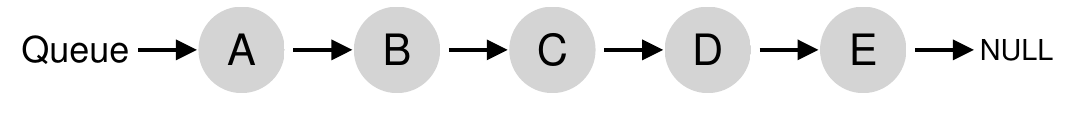
\includegraphics[width=1.\textwidth]{single-queue}
	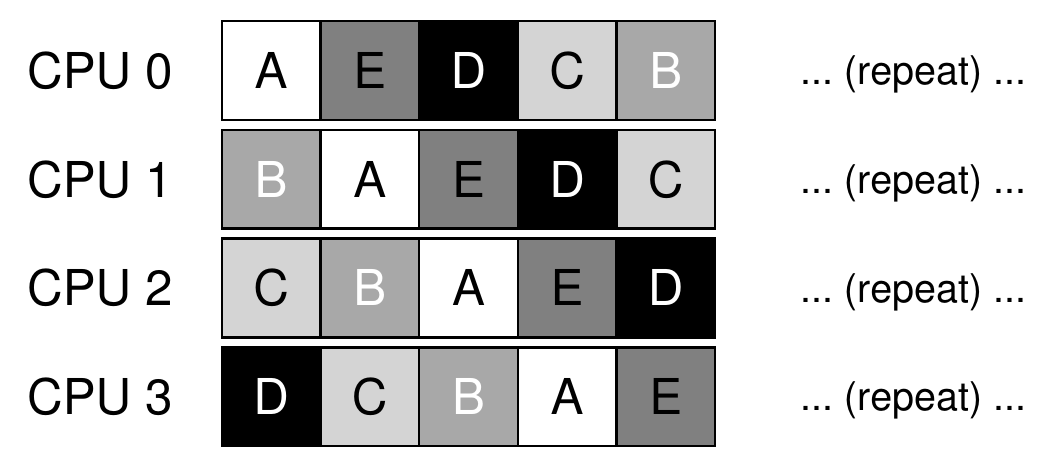
\includegraphics[width=1.\textwidth]{sqms}	
	\end{column}
	
	\begin{column}{.5\textwidth}
		\large
		最基本的方式是简单地复用单处理器调度的基本架构,将所有需要调度的工作放入 一个单独的队列中,我们称之为单队列多处理器调度(Single Queue Multiprocessor Scheduling,SQMS)。

		
	\end{column}
\end{columns}
\end{frame}
%%------------------------------------------------
\begin{frame}
	\begin{columns}
		\begin{column}{.5\textwidth}
			\Large \centering
			单队列调度
			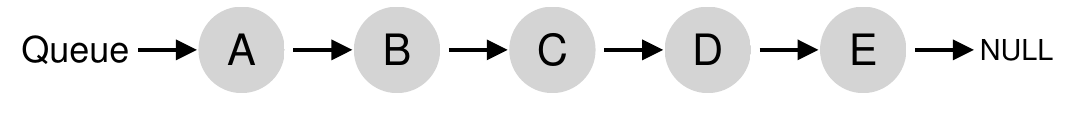
\includegraphics[width=1.\textwidth]{single-queue}
			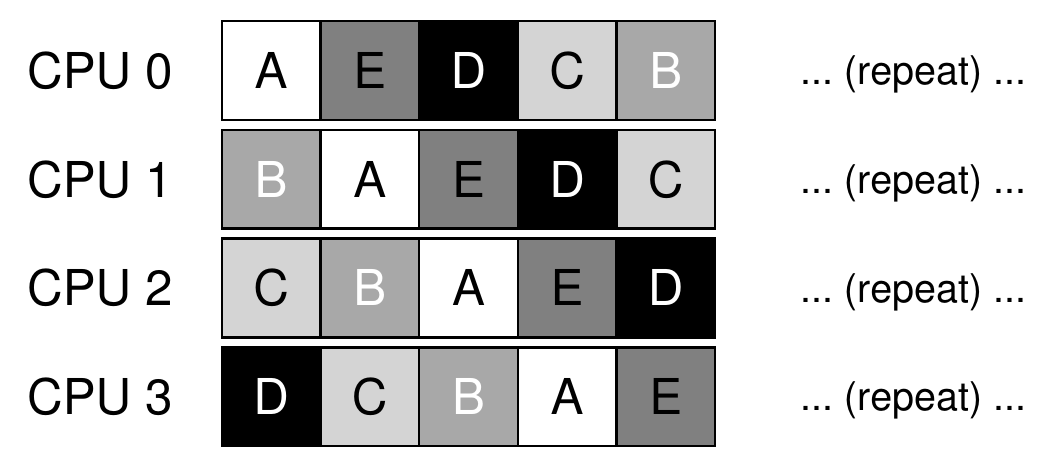
\includegraphics[width=1.\textwidth]{sqms}	
		\end{column}
		
		\begin{column}{.5\textwidth}
			\large
			单队列多处理器调度(SQMS)
			

			\begin{itemize}\large
				\item 缺乏可扩展性(scalability)
				\item 缓存亲和性(cache affinity)弱
			\end{itemize}
			
		\end{column}
	\end{columns}
\end{frame}


%%------------------------------------------------
\begin{frame}
	\begin{columns}
		\begin{column}{.5\textwidth}
			\Large \centering
			单队列调度
			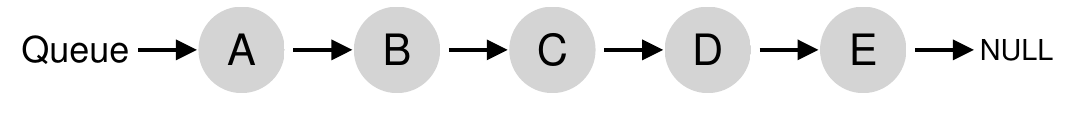
\includegraphics[width=1.\textwidth]{single-queue}
			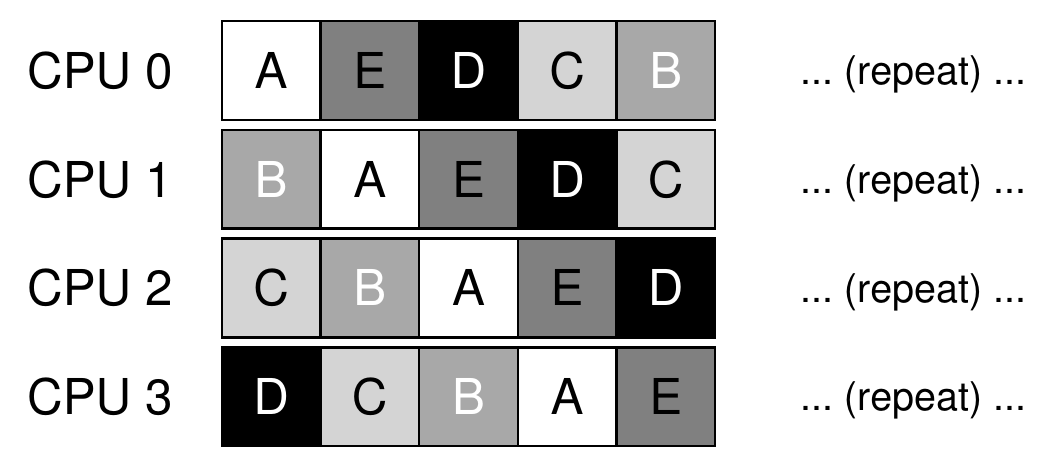
\includegraphics[width=1.\textwidth]{sqms}	
		\end{column}
		
		\begin{column}{.5\textwidth}
			\large
			单队列多处理器调度(SQMS) \\
			\normalsize
			尽可能让进程在同一个CPU上运行。保持一些工作的亲和度的同时,可能需要牺牲其他工作的亲和度来实现负载均衡。
			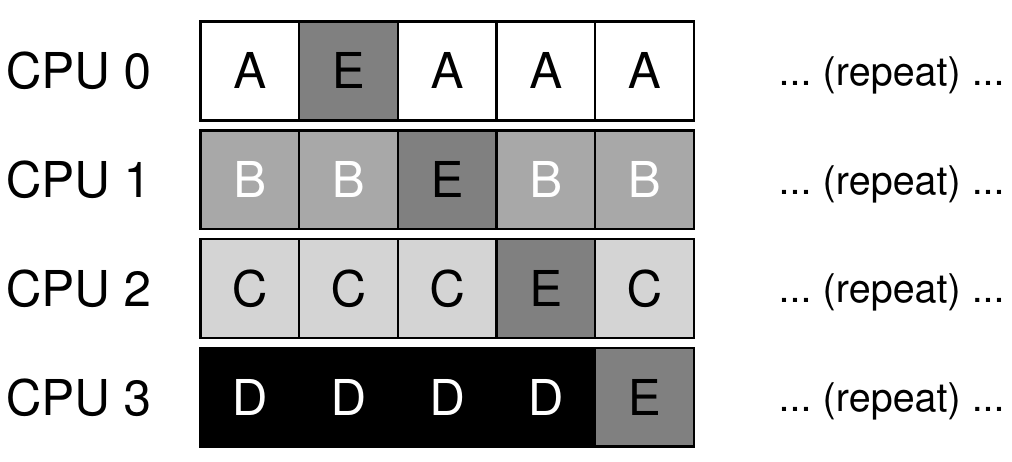
\includegraphics[width=1.\textwidth]{sqms-cache-affinity}

			
		\end{column}
	\end{columns}
\end{frame}

%%------------------------------------------------
\begin{frame}
	\begin{columns}
		\begin{column}{.5\textwidth}
			\Large \centering
			多队列调度
			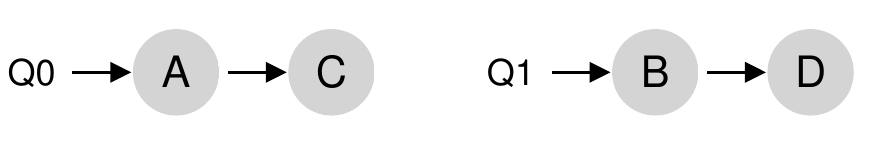
\includegraphics[width=1.\textwidth]{multi-queue}
			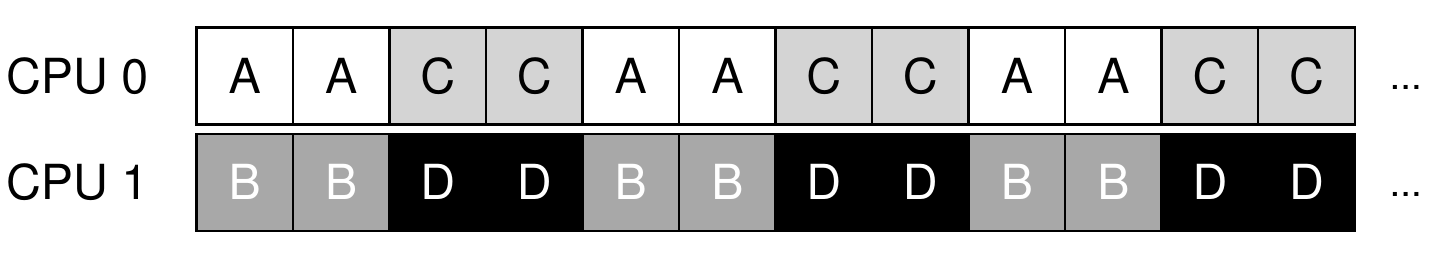
\includegraphics[width=1.\textwidth]{mqms}	
		\end{column}
		
		\begin{column}{.5\textwidth}
			\large
			多队列多处理器调度(Multi-Queue Multiprocessor Scheduling,MQMS) \\
			\normalsize
			\begin{itemize}
			\item 在MQMS中,基本调度框架包含多个调度队列,每个队列可以使用不同的调度规则,比如轮转或其他任何可能的算法。
			
			\item 当一个工作进入系统后,系统会依照 一些启发性规则(如随机或选择较空的队列)将其放入某个调度队列。这样一来,每个CPU调度之间相互独立,就避免了单队列的方式中由于数据共享及同步带来的问题。
			\end{itemize}
		\end{column}
	\end{columns}
\end{frame}


%%------------------------------------------------
\begin{frame}
	\begin{columns}
		\begin{column}{.5\textwidth}
			\Large \centering
			多队列调度
			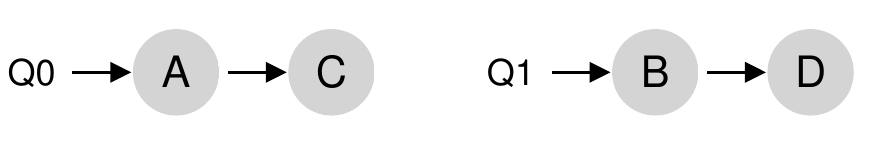
\includegraphics[width=1.\textwidth]{multi-queue}
			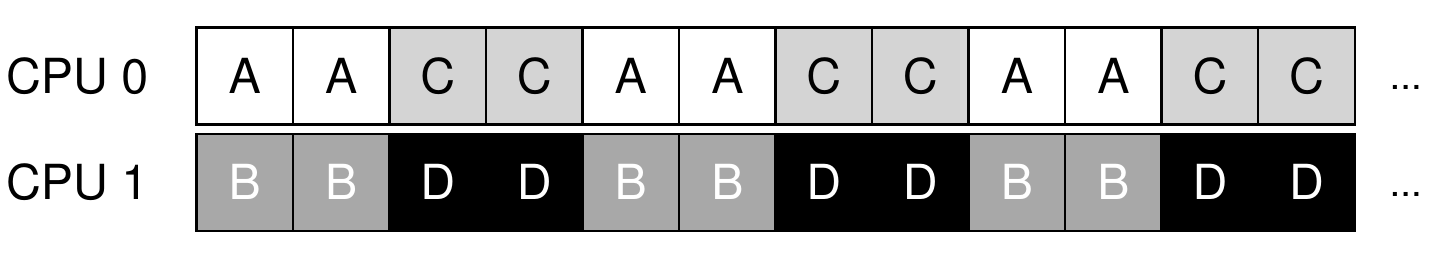
\includegraphics[width=1.\textwidth]{mqms}	
		\end{column}
		
		\begin{column}{.5\textwidth}
			\large
			多队列多处理器调度(MQMS) 
			\normalsize
			\begin{itemize}
			\item 根据不同队列的调度策略,每个CPU从两个工作中选择,决定谁将运行。例如,轮转调度
			\item 具有可扩展性。队列的数量会随着CPU的增加而增加,因此锁和缓存争用的开销不是大问题。
			\item 具有良好的缓存亲和度。所有工作都保持在固定的CPU上,因而可以很好地利用缓存数据。
			\end{itemize}
		\end{column}
	\end{columns}
\end{frame}


%%------------------------------------------------
\begin{frame}
	\begin{columns}
		\begin{column}{.5\textwidth}
			\Large \centering
			多队列调度
			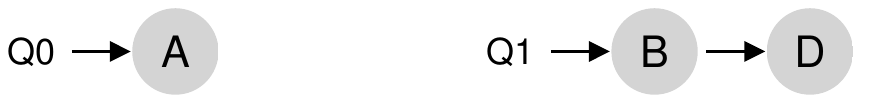
\includegraphics[width=1.\textwidth]{mqms-problem-1}
			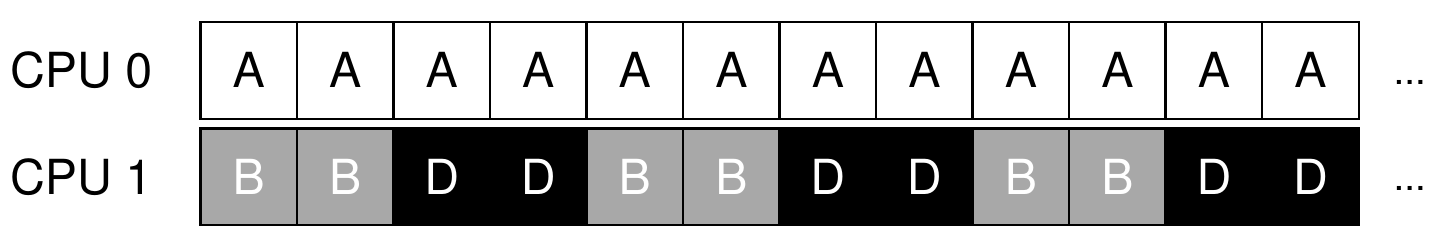
\includegraphics[width=1.\textwidth]{mqms-problem-2}	
		\end{column}
		
		\begin{column}{.5\textwidth}
			\large
			多队列多处理器调度(MQMS) \\
			负载不均(load imbalance) \\ 
			\normalsize
			假定和上面设定一样(4个工作,2个CPU),但假设一个工作(如C)这时执行完毕。如果对系统中每个队列都执行轮转调度策略:
			
			\begin{itemize}
				\item A获得了B和D两倍的CPU时间

			\end{itemize}
		\end{column}
	\end{columns}
\end{frame}

%----------------------------------------------


%%------------------------------------------------
\begin{frame}
	\begin{columns}
		\begin{column}{.5\textwidth}
			\Large \centering
			多队列调度
			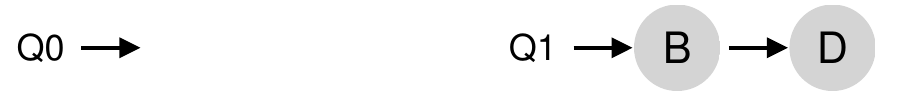
\includegraphics[width=1.\textwidth]{mqms-problem-3}
			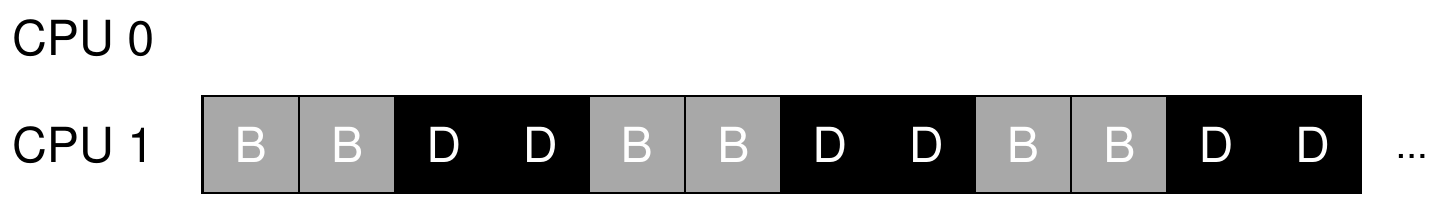
\includegraphics[width=1.\textwidth]{mqms-problem-4}	
		\end{column}
		
		\begin{column}{.5\textwidth}
			\large
			多队列多处理器调度(MQMS) \\
			负载不均(load imbalance) \\ 
			\normalsize
			假定和上面设定一样(4个工作,2个CPU),但假设A和C都执行完毕,系统中只有B和D。如果对系统中每个队列都执行轮转调度策略:
			
			\begin{itemize}
				\item CPU1很忙
				\item CPU0空闲
				
			\end{itemize}
		\Large
		怎样才能克服潜伏的负载不均问题?
		\end{column}
	\end{columns}
\end{frame}



%%------------------------------------------------
\begin{frame}
	\begin{columns}
		\begin{column}{.5\textwidth}
			\Large \centering
			多队列调度
			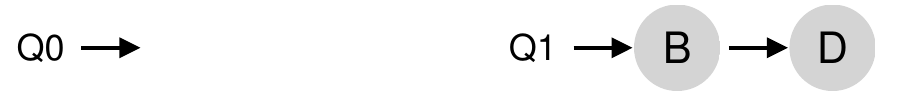
\includegraphics[width=1.\textwidth]{mqms-problem-3}
			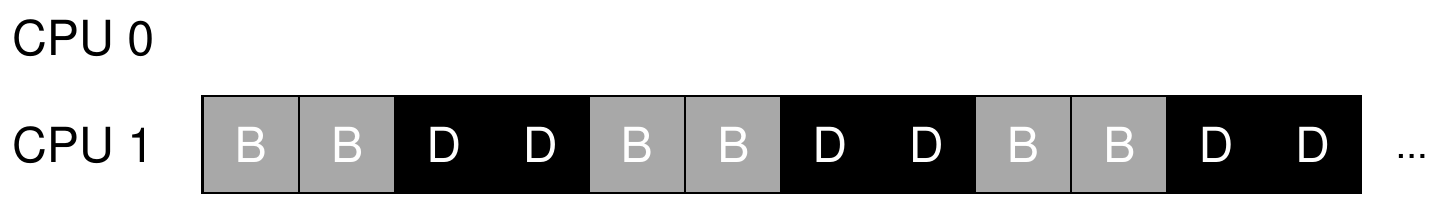
\includegraphics[width=1.\textwidth]{mqms-problem-4}	
		\end{column}
		
		\begin{column}{.5\textwidth}
			\large
			\begin{block}{关键问题:如何应对负载不均}
			多队列多处理器调度程序应该如何处理负载不均问题,从而更好地实现预期的调度目标?
			\end{block} 
			\normalsize
			最明显的答案是让工作移动,这种技术我们称为迁移(migration)。通过工作的跨CPU迁移,可以真正实现负载均衡。
			
			\begin{itemize}
				\item 情况:有一个CPU空闲,另一个CPU有一些工作。
				\item 迁移:将B或D迁移到CPU0。
		
			\end{itemize}
			\Large

		\end{column}
	\end{columns}
\end{frame}



%%------------------------------------------------
\begin{frame}
	\begin{columns}
		\begin{column}{.5\textwidth}
			\Large \centering
			多队列调度
			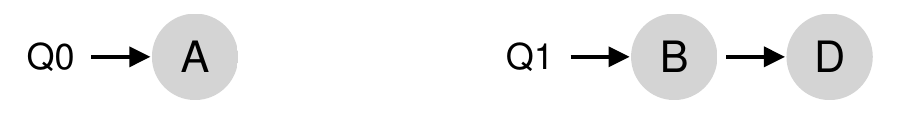
\includegraphics[width=1.\textwidth]{mqms-problem-5}
			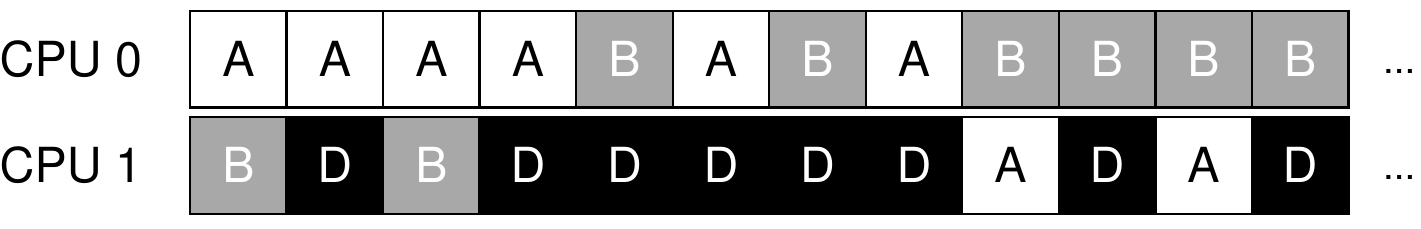
\includegraphics[width=1.\textwidth]{mqms-problem-6}	
		\end{column}
		
		\begin{column}{.5\textwidth}
			\large
			\begin{block}{关键问题:如何应对负载不均}
				多队列多处理器调度程序应该如何处理负载不均问题,从而更好地实现预期的调度目标?
			\end{block} 
			\normalsize
			最明显的答案是让工作移动,这种技术我们称为迁移(migration)。通过工作的跨CPU迁移,可以真正实现负载均衡。
			
			\begin{itemize}
				\item 情况:A独自留在CPU 0上,B和D在CPU 1上交替运行。
				\item 迁移:不断地迁移和切换一个或多个工作。
				
			\end{itemize}
		\large
		系统如何决定发起这样的迁移?
			\Large
			
		\end{column}
	\end{columns}
\end{frame}
%----------------------------------------------





\end{document}
